\section{Evaluation}

For evaluation, we deploy Giza on top of the Microsoft Azure platform across 11 data centers (7 in North America, 2 in Europe and 2 in Asia). Giza nodes are Azure virtual machines with 16 cores, 56 GB of RAM, and Gigabit Ethernet. As describe in Section~\ref{sec:design}, all the Giza nodes are stateless. For each Giza storage account, a locally redundant Azure Blob and Table storage account is created in every DC. Upon receiving {\em get} or {\em put} requests, the Giza nodes execute the data and the metadata paths to read or write objects.

\begin{figure*}
\begin{tabular}{c|c|c|c|c|c}
& coding rate & \# of DCs & DC location & Max Metadata Latency & Max Latency\\
\hline
US-2-1 & 2+1 & 4 & Central, South Central, West & 40 ms& 40 ms\\
US-6-1 & 6+1 & 8 & Central, South Central, West&?? 40 ms&?? 42 ms\\ 
world-2-1 & 2+1 & 4 & Central, Europe North, Japan East & 140 ms & 140 ms\\
world-6-1 & 6+1 & 8 & Central, South Central, West & 40 ms & 140 ms\\
\end{tabular}
\caption{The DC configurations and inter-DC latencies in various experiments~\label{fig:dcconfig}} 
\end{figure*}

\subsection{Setup}
Our experiments involve a varying number of DCs in different configurations. In
each DC, we deploy a single Azure virtual machine (16 cores, 56 GB of RAM, and
gigabit ethernet) and create a storage account for accessing Azure blob and
table storage. Both the blob and table storage are configured with the
``locally redundant'' replication level.  Each \name node accesses the local
DC's cloud storage and also proxies the storage requests from \name nodes in
other DCs.  

For CockroachDB experiments, we run a CockroachDB cluster spanning across
multiple DCs.  We use the same set of Azure virtual machines and run a single
CockroachDB node per DC. Our configuration of CockroachDB follows the
recommended production settings by the developers of CockroachDB. For example,
we run NTP to synchronize the clocks of different CockroachDB nodes. 

We generate experimental workloads using the YCSB benchmark. In the generated
workload, the probability of accessing a given key follows a Zipf distribution.
We experiment with different object sizes ranging from 128KB to 4MB. 

We experiment with four diffferent DC configurations, as shown in
Figure~\ref{fig:dcconfig}.  These configurations correspond to different coding
rates and different choices of DCs, either within US-only or spread across the
world. The wide-area latency across different DCs plays an important role in 
the performance of \name.  Figure~\ref{fig:dcconfig} reports the majority
latency (measured as the latency required to get a response from a majority
quorum of DCs) and the maximum latency between DCs.



\subsection{Metadata Latency}

We implement Giza's metadata path with both Classic and Fast Paxos. Here, we compare the performance of the two algorithms and examine their effects on Giza's metadata path latency. Figure~\ref{fig:metadata} presents the metadata latencies and breakdowns for both US-2-1 and World-2-1 configurations. The results include running proposers in each of the DCs.

The metadata latency consists of three parts: query version latency, transfer latency, and table latency.
The query version latency is determined by reading the possible highest version from the proposer’s local table. This request is not part of the concensus protocol and is the same for both Fast and Classic Paxos.
The transfer latency is the amount of time spent on network communication between the proposer and the furthest Giza proxy in a Paxos quorum. Here, the latency of Classic Paxos, which incurs two cross-DC round trips, is not strictly twice as much as the latency of Fast Paxos. This is because the Classic Paxos quorum is smaller than the Fast Paxos quorum. As a result, the distance between the proposer and the {\em furthest} proxy is smaller in a Classic Paxos quorum.
The table latency is the latency for a Giza proxy to conditionally update its local DC table. Since Classic Paxos requires two rounds and hence two table updates, its table latency is twice that of Fast Paxos.

%The metadata latency is first affected by the number of cross-DC round trips the Paxos algorithms require. Classic Paxos takes 2 cross-DC round trips and Fast Paxos only 1 round trip. The latency of single round trip consists of two parts: 1) transfer latency, which is the latency to relay the metadata request to a proxy Giza node in a remote DC; and 2) table latency, which is the latency to conditionally update the table locally in the remote DC.

%It turns out that the table latencies across various DCs are quite comparable, around 60 ms or so.
%The transfer latencies, however, vary significantly from 20 ms (US central to US south central) to 240 ms (east Japan to north Europe).
%
%The metadata latency is further affected by quorum size. Classic Paxos completes with 2 out of 3 
%
%Indeed, Figure~\ref{fig:metadata} presents the metadata latencies and breakdowns for the both US-2-1 and World-2-1 configurations.

%When comparing the performance between implementing the metadata path with Fast Paxos and Classic Paxos, we found two factors that are important in determining which configuration outperforms the other.  The first factor is whether the VM to local Azure write latency is dominant in the metadata path and the second factor is the difference in the maximal distance between data centers in a fast quorum and a classic quorum. 
%
%The performance of the metadata path is primarily determined by the request latency between the coordinator and the table storage of the furthest data center in the quorum. Each request to a remote table storage is broken down into two parts: VM to VM latency and VM to local Azure storage latency. From our previous analysis, the write latency from a VM to its local Azure storage is around 60 ms. The VM to VM latency is determined by the location of the data centers and can range from 20 ms (us central to us south central) to 240 ms (east Japan to north Europe). Figure~\ref{fig:metadata} illustrates the latency difference between the two Paxos schemes.

For the US-2-1 configuration, we observe that the metadata latency is dominated by table latency. In this case, Fast Paxos is much faster than Classic Paxos, regardless of the proposer's location.

For the World-2-1 configuration, transfer latency becomes a substantial part of the overall metadata latency. In this case, despite of taking two cross-DC round trips, the Classic Paxos implementation can have lower transfer latency. Nevertheless, the table latency of Classic Paxos is still twice that of Fast Paxos. As a result, the Fast Paxos implementation has lower latency, regardless of the proposer's location.

%In addition, if the max distance between the data centers in a fast quorum is close to that in a classic quorum, the latency of the Fast Paxos metadata path is half of that of the Classic Paxos metadata path. In certain scenarios, it is possible for Classic Paxos to achieve lower latency than Fast Paxos. While we didn’t observe this in our two configurations, we see that if we start the request from North Europe in the 2-1 world configuration, the latencies are almost the same. This is because a Fast Paxos round requires a bigger quorum response and in this case, a fast quorum consists of North Europe, US, and East Japan. The VM to VM latency between North Europe and East Japan is 240 ms while the VM to VM latency between North Europe and US is only 102 ms. Hence the max distance between data centers in the classic quorum (US and North Europe) is less than half of that of the fast quorum. The scenario in which the Classic Paxos scheme outperforms the Fast Paxos scheme is:
%\[max\_dist(F) > 2 * max\_dist(Q) + \textrm{extra table access}
%\]
%where F is the fast quorum size and Q is the classic quorum size.
\begin{figure}[t]
%  \centerline {
      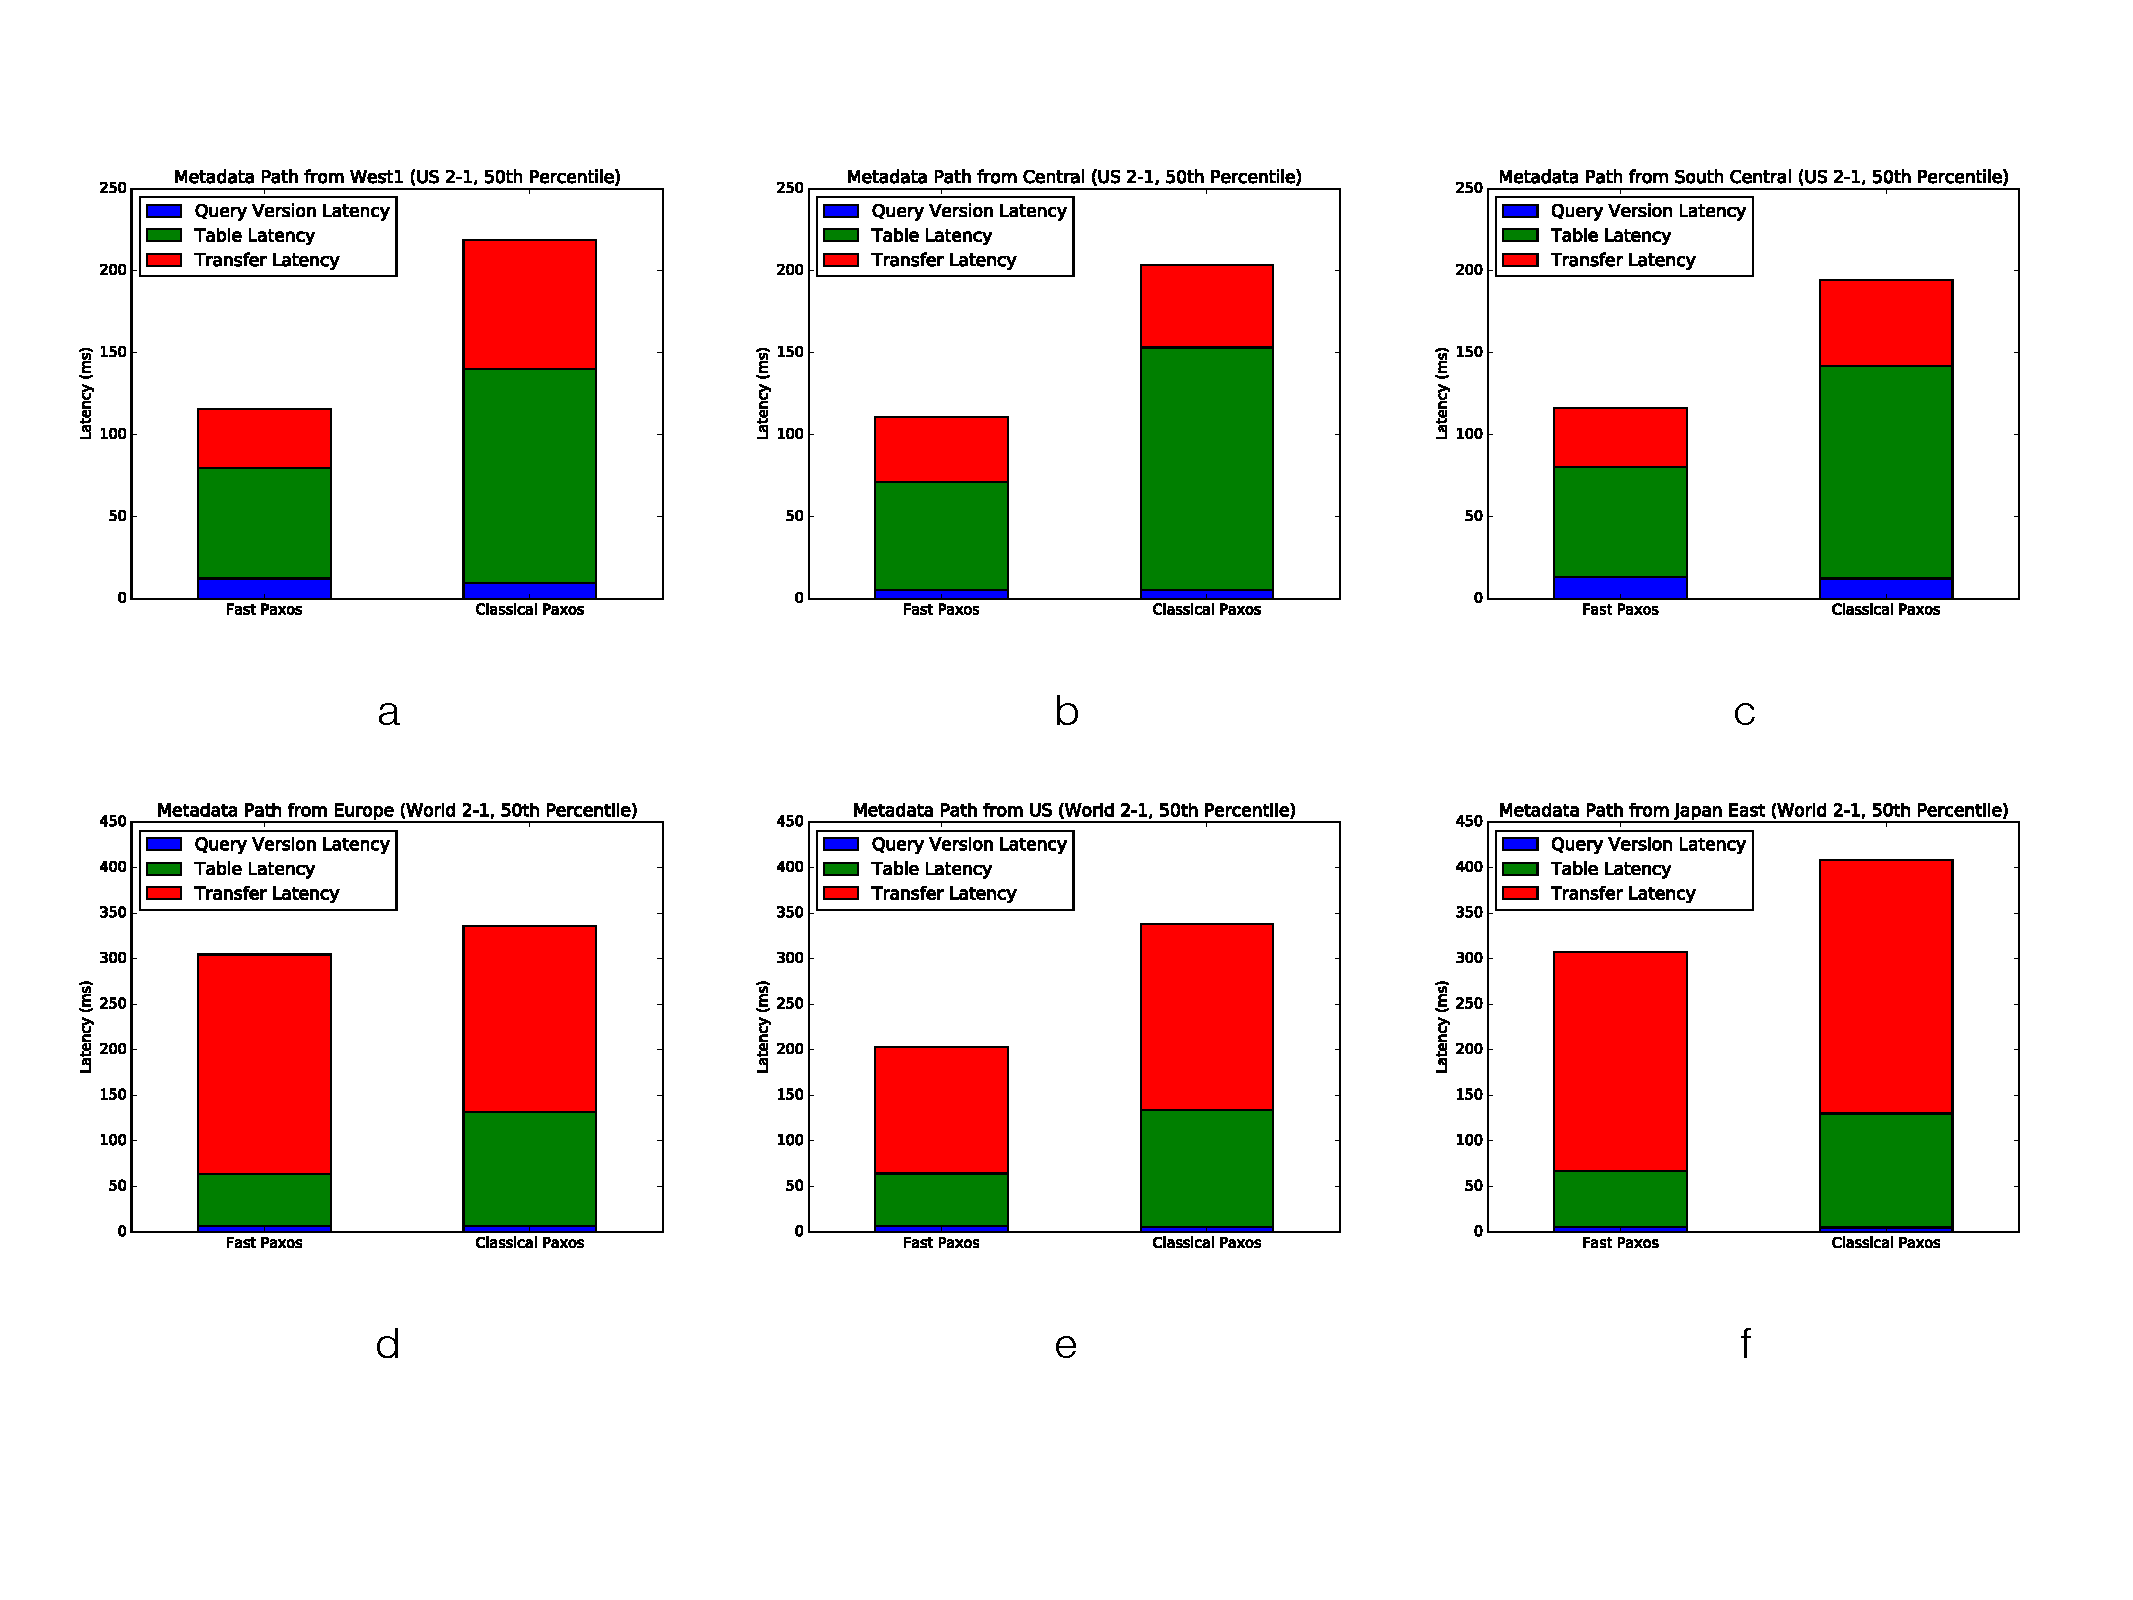
\includegraphics[width=\linewidth]{images/Metadata_vs}
      \caption{Fast Paxos and Classic Paxos Comparison}
      \label{fig:metadata}
%  }
\end{figure}


\subsection{\name Latency}

The design of Giza went through multiple iterations and this section illustrates the performance gain in latency for each iteration. For the interest of space, we focus on the World-2-1 configuration.
%where US Central generates all requests as representative of the performance gain seen in other configurations.

\subsubsection{Giza {\em Put} Latency}
%\subsubsection{Giza Latency}

%\begin{figure}[t]
%  \centerline {
%    \begin{subfigure}{0.20\textwidth}
%      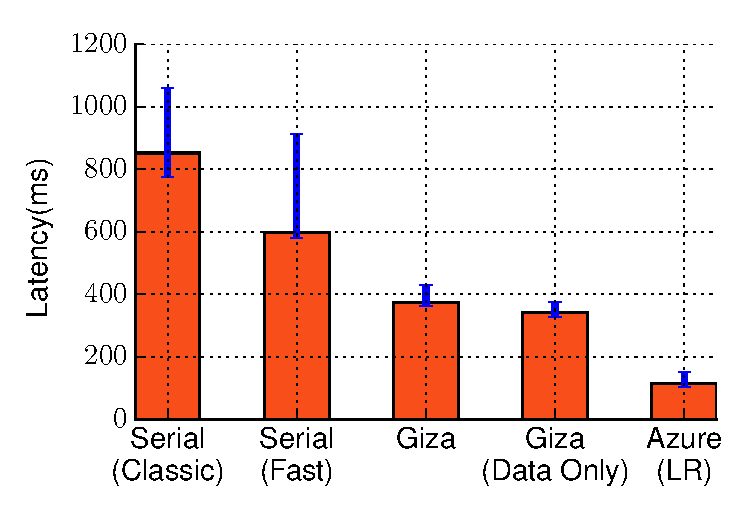
\includegraphics[width=\linewidth]{plots/giza_lat_put}
%      \caption{Put}
%      \label{fig:eval_giza_put}
%    \end{subfigure}
%    \begin{subfigure}{0.20\textwidth}
%      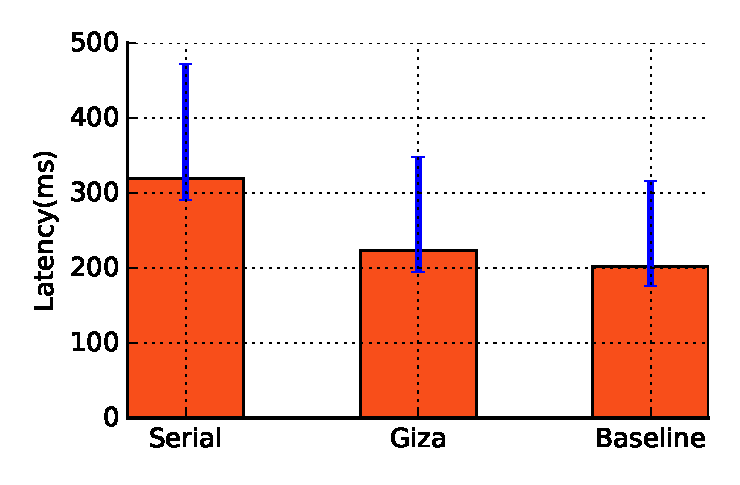
\includegraphics[width=\linewidth]{plots/giza_lat_get}
%      \caption{Get}
%      \label{fig:eval_giza_get}
%    \end{subfigure}
%  }
%  \caption{\name Overall Latency}
%  \label{fig:geo_tpcc}
%\end{figure}

%%% Local Variables:
%%% mode: latex
%%% TeX-master: "main"
%%% End:


Figure~\ref{fig:eval_giza_put} shows the \name overall {\em put} latency for 4MB data. We compare Giza with its two previous iterations where the metadata path is not parallelized with the data path. In the first iteration, Giza runs the data path first. After completing the data path, Giza runs the metadata path with the Classic Paxos implementation. In the second iteration, we replaced Classic Paxos with Fast Paxos, improving latency performance. Giza parallelizes metadata path with data path, which can results in extra metadata or data clean up if either path fails to complete. However, the performance gain is significant. We also included a baseline which is the time it takes a proposing data center to issue a blob store request to the farthest data center in the quorum. Finally, we include the latency for storing the 4MB data directly to Azure storage, which is locally replicated.

The results show that \name's performance beats the other two alternatives in the common case and has closest
latency to the baseline. The median latency of \name's {\em put} is 374 ms, which is only 30 ms
higher than the baseline. This is due to the latency of erasure coding 4MB data. On the other hand, the serial classic paxos version takes 
852 ms, and the serial fast paxos version takes 598 ms. In summary, the latency cost for tolerating data center failure with Giza is a little more than 3 time that of local replication.

\subsubsection{Giza {\em Get} Latency}

Figure~\ref{fig:eval_giza_get} shows Giza's {\em get} performance comparison. The alternative design here is the non-optimistic {\em get } where the most current version for a blob is not assumed to be stored in the current data center. Hence, the metadata path and data path are executed sequentially, taking 419 ms. Giza's optimistic {\em get}, which runs the metadata path and data path in parallel, takes 223ms. Giza's {\em get} latency is higher than the baseline by 33 ms. The performance gap between \name and baseline is higher because \name needs to do a local table retrieval first before starting the datapath. In addition, it needs to decode the data fragments. Here the latency cost of erasure encoding on the read path with Giza is roughly twice that of reading from a locally redundant Azure storage.

%The results are expected. The \name put latency consists of a 
%metadata put latency and datapath latency. 



\comment{

% \begin{figure}[!h]
% \centering
%   \subfloat[Giza Put 99th Percentile]{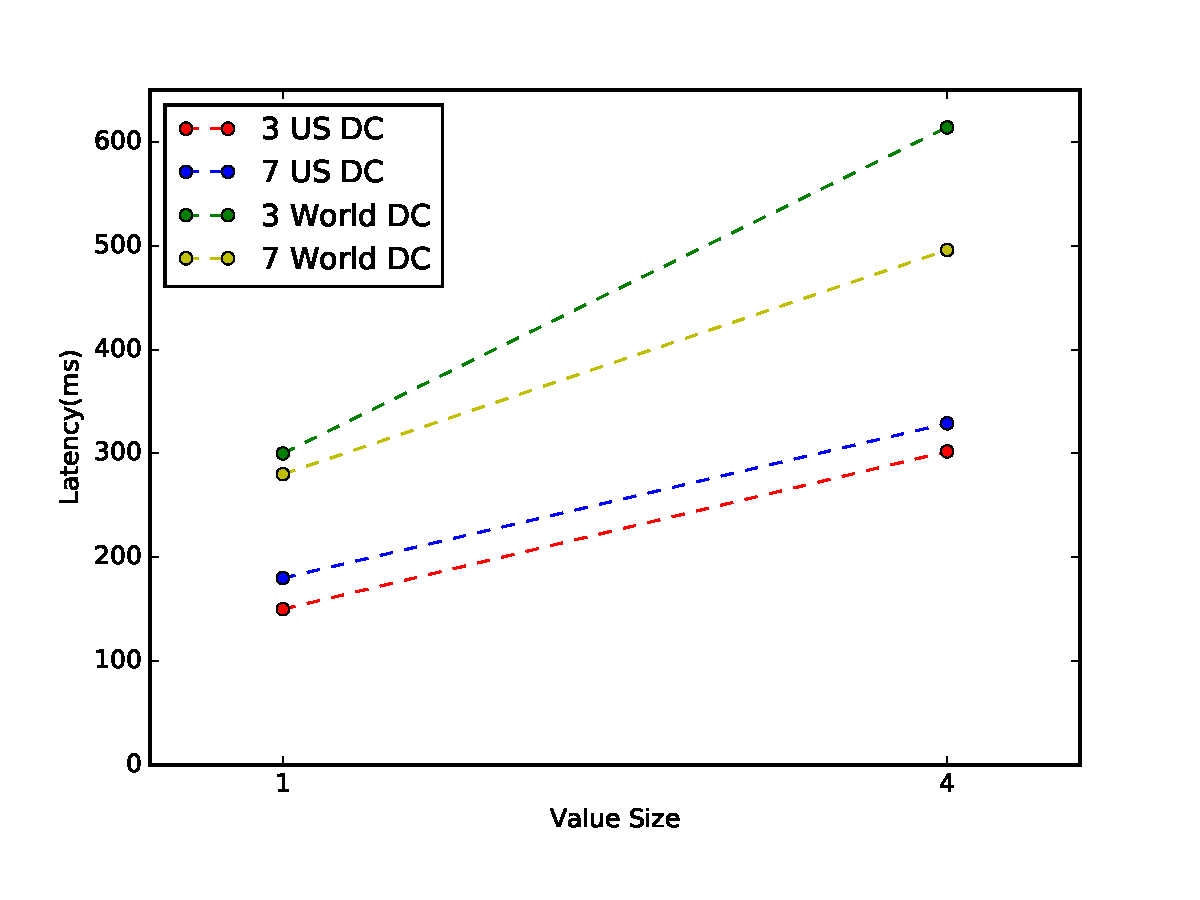
\includegraphics[width=0.5\textwidth]{images/write_latency}\label{fig:f1}}
%   \subfloat[Giza Get 99th Percentile]{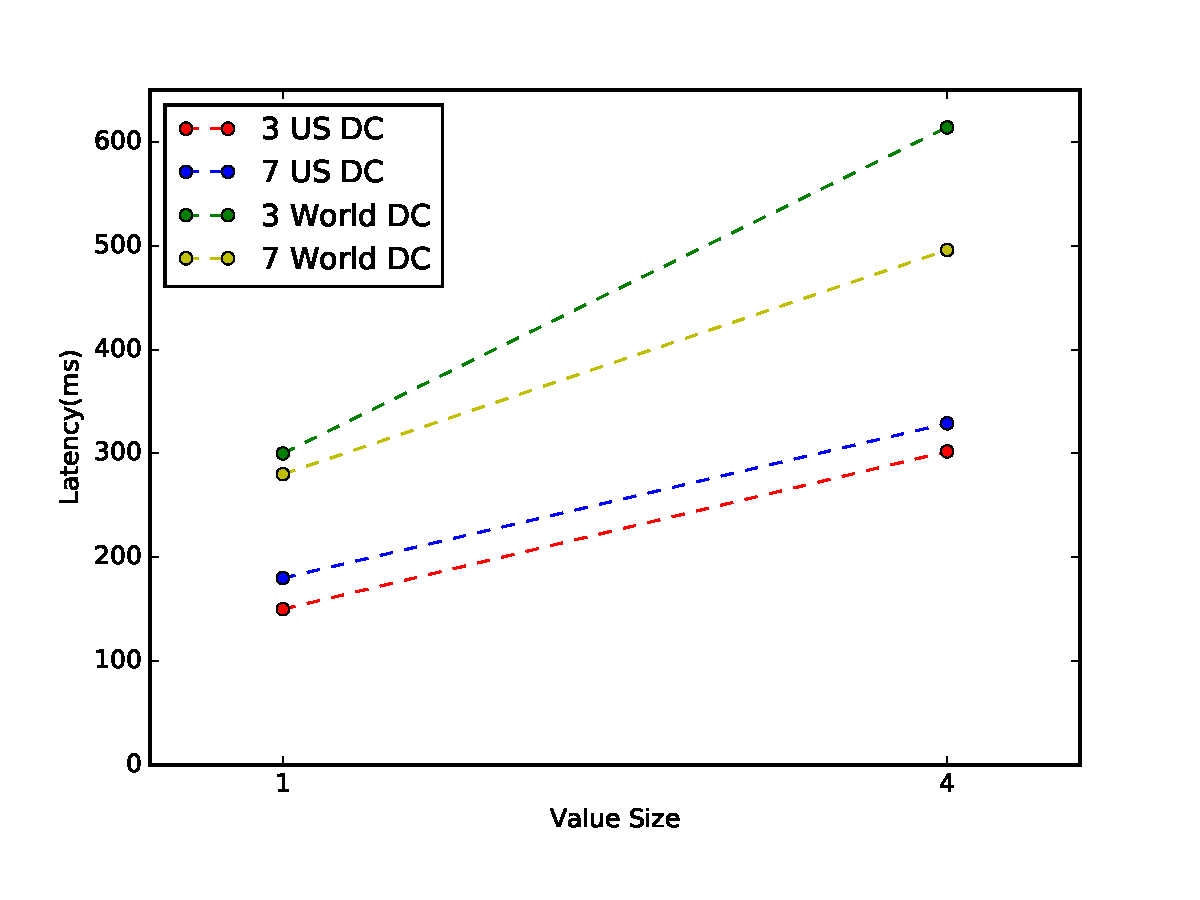
\includegraphics[width=0.5\textwidth]{images/write_latency}\label{fig:f2}}
% \caption{Comparison of latency of the four configurations}
% \end{figure}
\subsection {Different Configurations}
\sm {
  In this section, I will provide a latency graph (put and get) of all the 4 different configurations. The x axis is the size of the objects and the y axis is the latency. This section is to illustrate the trade off between storage efficiency and read latency. 
}

}

\subsection{Footprint Impact}


\begin{figure}[t]
%  \centerline {
    \begin{subfigure}{0.40\textwidth}
      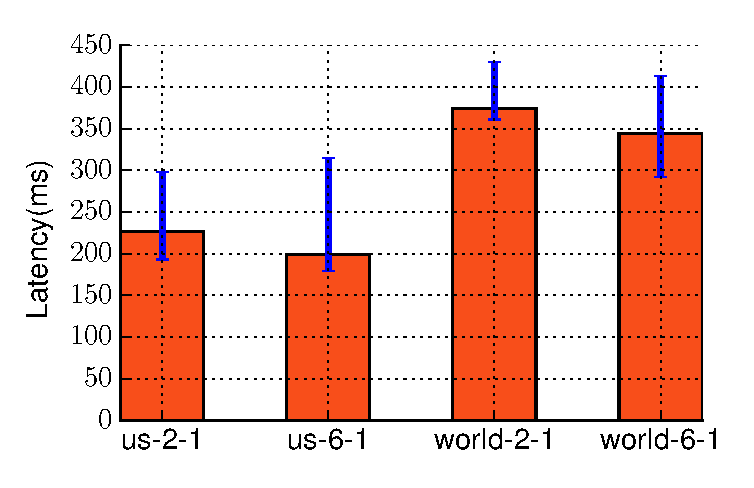
\includegraphics[width=\linewidth]{plots/giza_four_put}

      % \placeholder{
      %   x-axis: \# clients / partition\\
      %   y-axis: cluster throughput\\
      %   lines: \name{}, OCC, 2PL, TAPIR\\
      %   }
%                \vspace{-1\baselineskip}
      \caption{Put}
      \label{fig:eval_giza_put_four}
    \end{subfigure}
%    \begin{subfigure}{0.33\textwidth}
%      \includegraphics[width=\linewidth]{figs/graphs/multi_dc/tpcc/tpcc_NEW_ORDER_tpcc_client_lat90.eps}
%
%      % \placeholder{
%      %   x-axis: \# clients / partition\\
%      %   y-axis: latency (median, p90, p99)\\
%      %   (maybe only show median and p99 or just median and report typical distribution)\\
%      %   lines: \name{}, OCC, 2PL, TAPIR\\
%      % }
%      \caption{90\% Latency}
%      \label{fig:geo_tpcc_latency}
%    \end{subfigure}
    \begin{subfigure}{0.40\textwidth}
      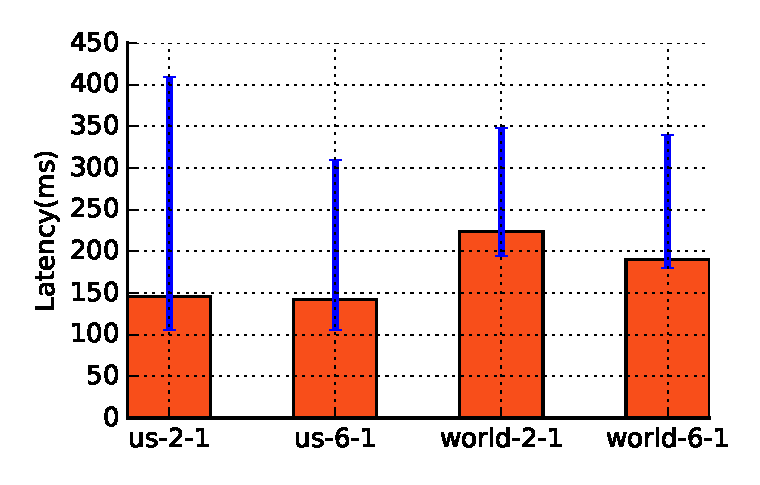
\includegraphics[width=\linewidth]{plots/giza_four_get}

      % \placeholder{
      %   x-axis: \# clients / partition\\
      %   y-axis: commit rate\\
      %   lines: \name{}, OCC, 2PL, TAPIR\\
      % }
      %\includegraphics[width=\linewidth]{fig/kodiak/tpcc_mix_10_nlog_ct_cr.pdf}
%                \vspace{-1\baselineskip}
      \caption{Get}
      \label{fig:eval_giza_get_four}
    \end{subfigure}
%  }
  \caption{Performance for \name in different setups}
\end{figure}

%%% Local Variables:
%%% mode: latex
%%% TeX-master: "main"
%%% End:


\name offers customers the flexibility to choose the set of data centers, as well as the erasure coding parameters (e.g., the number of data fragments $k$). 
%As the main goal of Giza is storage cost reduction, we want to encourage erasure encoding with more numbers of data fragments.
It turns out that increasing $k$ not only reduces storage overhead, but also overall latency. This is because the latency in Giza is often dominated by the data path. Erasure coding with a larger $k$ results in smaller fragments and fewer bytes stored in each DC's blob storage. This reduces the data path latency and in turn the overall latency.

Figure~\ref{fig:eval_giza_put_four} and Figure~\ref{fig:eval_giza_get_four} present the latency impact given different Giza footprints and erasure coding parameters. All the requests are generated from US-Central. Comparing US-2-1 to US-6-1 (World-2-1 to World-6-1), it is clear that increasing $k$ from 2 to 6 reduces the latency for both {\em put} and {\em get}.
%This improvement of performance occurs when the max distance between the data centers in the higher configuration group (7 data centers) is not more than that in the lower configuration group (3 data centers).


\subsection{Comparing Giza with CockroachDB}

Ideally, we would like to compare Giza with an existing storage system with
similar functionalities.  However, there is no off-the-shelf erasure coded
system.  Hence, we implemented Giza on top of CockroachDB using its transaction support.
To do this, we create four different tables in CockroachDB: one metadata table
and three data tables (for storing coded fragments). The metadata table is
replicated across all three DCs. Each of the data tables is replicated three
times within its respective data center. This is to match the local
replication of Azure Table within individual DCs.  

We implement Giza's {\em put} as a transaction consisting of storing each coded
fragment at the corresponding data table and storing the metadata information
in the metadata table. Since CockroachDB is not optimized for storing large
objects, we evaluate the performance of {\em put}s on 128KB objects.  The
median {\em put} latency of 128KB objects under CockroachDB is 333ms, much
higher than that of Giza (<100ms).  

We implement Giza's {\em get} as a transaction consisting of reading the
metadata from the metadata table and two coded fragments from the data tables.
The median {\em get} latency under CockroachDB is lower than that of Giza by
20\%. This is because CockroachDB directly reads from local HDD,
which is faster than Giza reading from Azure storage. To demonstrate this, we
equalize the storage layer to substitute Azure latency with local HDD latency.
Indeed, Giza's performance with equalized storage is slightly better than that
of CockroachDB. 

%\begin{figure}[t]
%  \centerline {
    \begin{subfigure}{0.45\textwidth}
      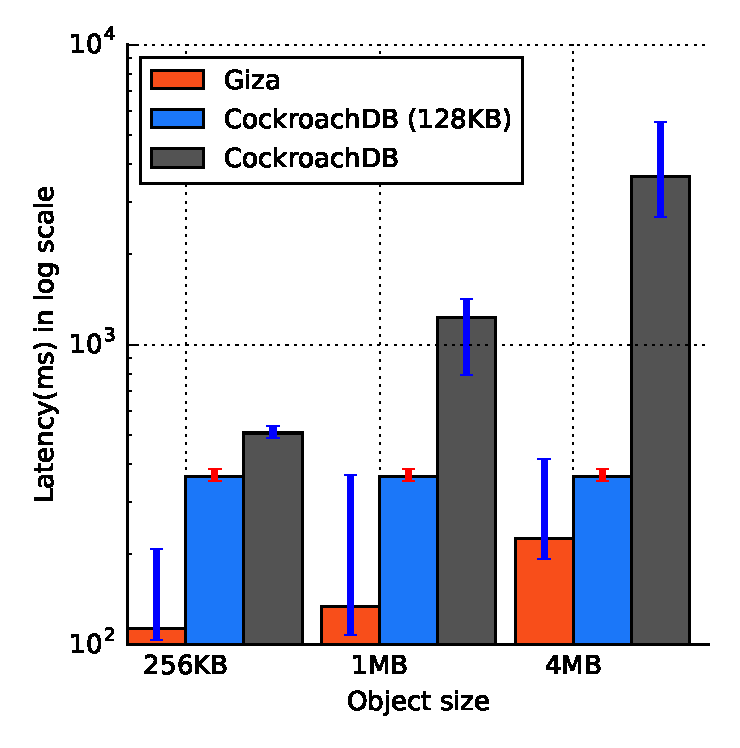
\includegraphics[width=\linewidth]{plots/giza_cock_put}

      % \placeholder{
      %   x-axis: \# clients / partition\\
      %   y-axis: cluster throughput\\
      %   lines: \name{}, OCC, 2PL, TAPIR\\
      %   }
%                \vspace{-1\baselineskip}
      \caption{Put}
      \label{fig:eval_cock_put}
    \end{subfigure}
%    \begin{subfigure}{0.33\textwidth}
%      \includegraphics[width=\linewidth]{figs/graphs/multi_dc/tpcc/tpcc_NEW_ORDER_tpcc_client_lat90.eps}
%
%      % \placeholder{
%      %   x-axis: \# clients / partition\\
%      %   y-axis: latency (median, p90, p99)\\
%      %   (maybe only show median and p99 or just median and report typical distribution)\\
%      %   lines: \name{}, OCC, 2PL, TAPIR\\
%      % }
%      \caption{90\% Latency}
%      \label{fig:geo_tpcc_latency}
%    \end{subfigure}
    \begin{subfigure}{0.45\textwidth}
      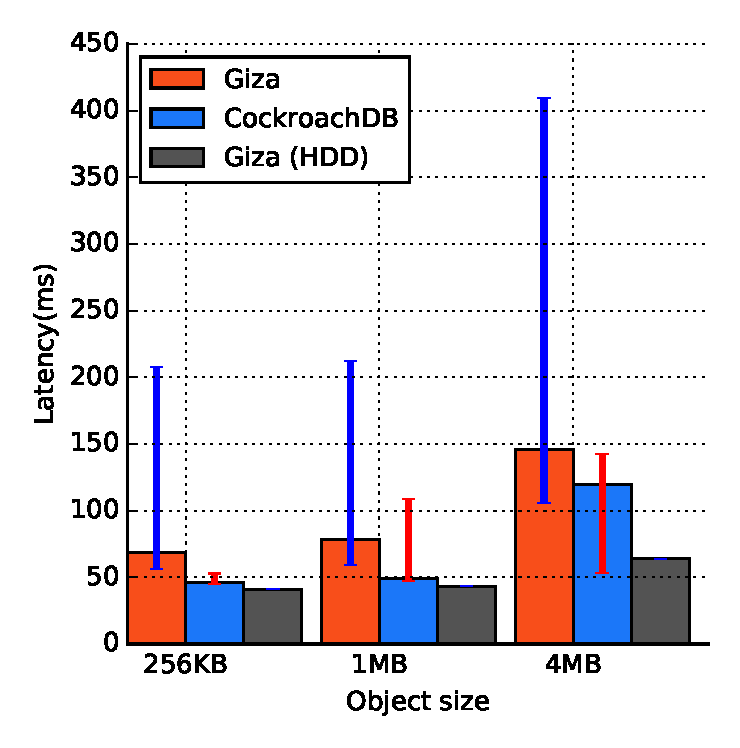
\includegraphics[width=\linewidth]{plots/giza_cock_get}

      % \placeholder{
      %   x-axis: \# clients / partition\\
      %   y-axis: commit rate\\
      %   lines: \name{}, OCC, 2PL, TAPIR\\
      % }
      %\includegraphics[width=\linewidth]{fig/kodiak/tpcc_mix_10_nlog_ct_cr.pdf}
%                \vspace{-1\baselineskip}
      \caption{Get}
      \label{fig:eval_cock_get}
    \end{subfigure}
%  }
  \caption{Performance for \name in different setups}
\end{figure}
% \begin{figure}[t]
% %  \centerline {
%       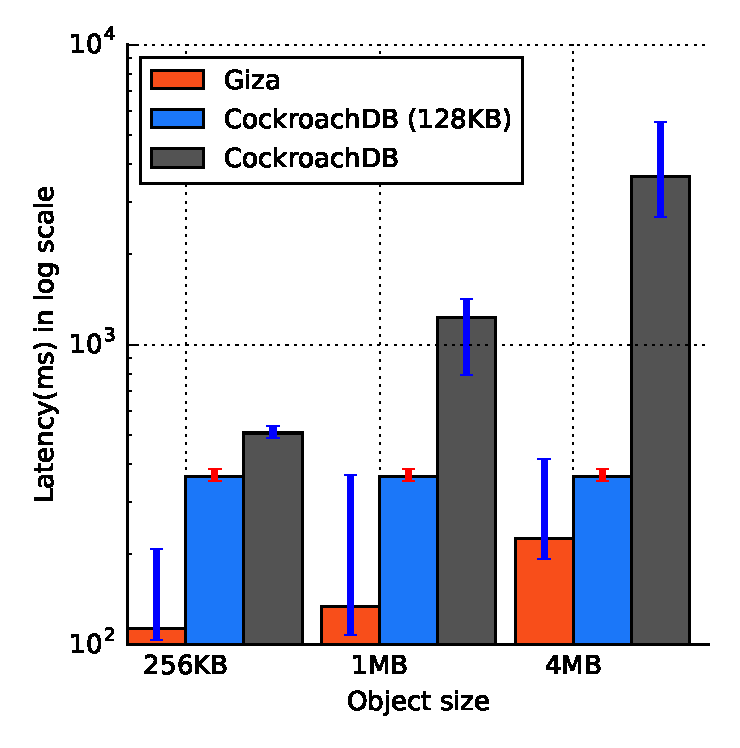
\includegraphics[width=\linewidth]{plots/giza_cock_put}
%       \caption{CockroachDB vs Giza Put with various object sizes}
%       \label{fig:eval_cock_put}
% %  }
% \end{figure}

% %\begin{figure}[t]
% %  \centerline {
% %      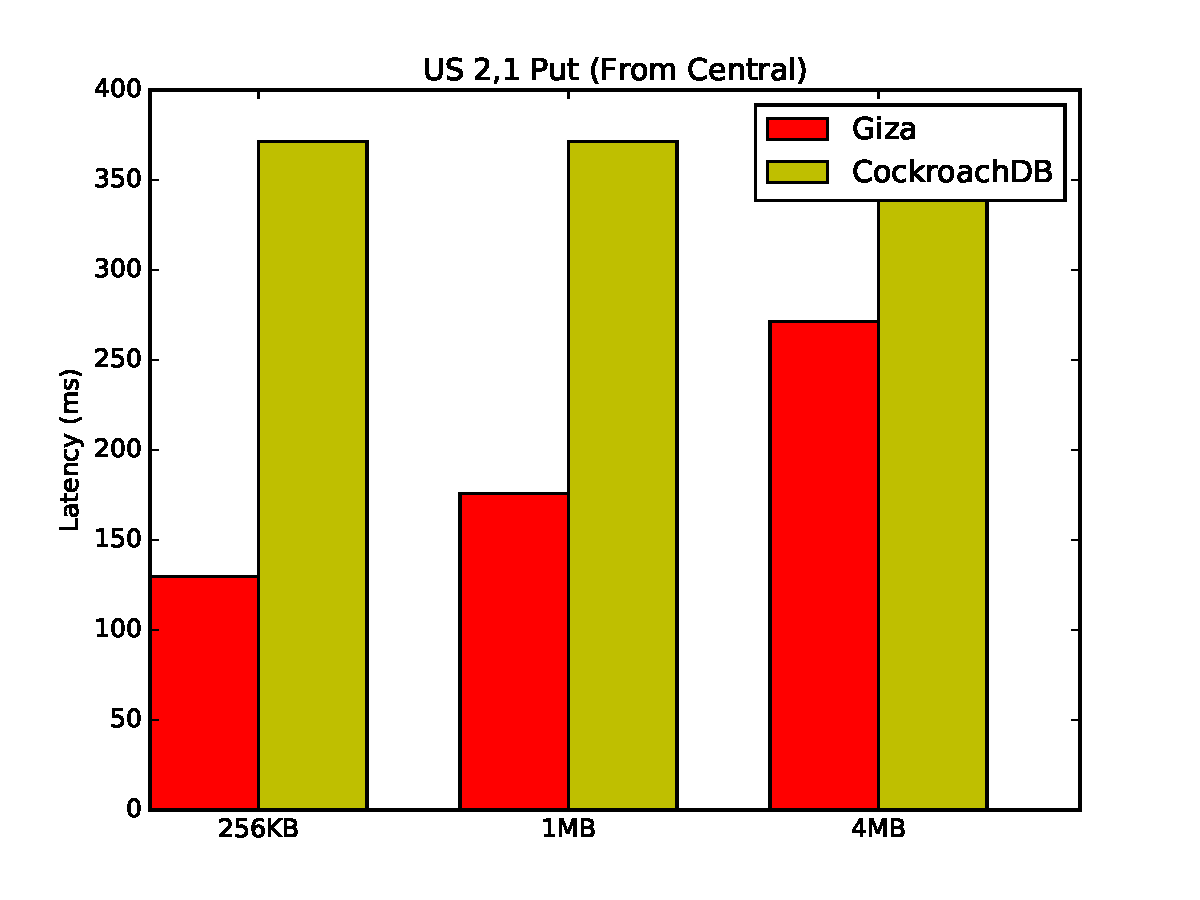
\includegraphics[width=\linewidth]{images/cockroach_vs_giza_put_128}
% %      \caption{CockroachDB vs Giza with various object sizes}
% %      \label{fig:eval_cock_put2}
% %  }
% %\end{figure}

% \begin{figure}[t]
% %  \centerline {
%       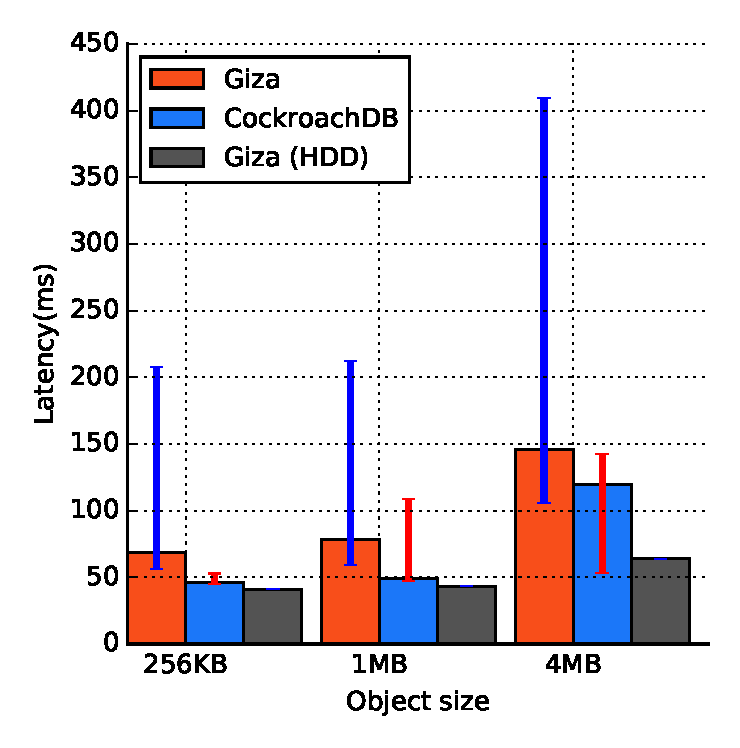
\includegraphics[width=\linewidth]{plots/giza_cock_get}
%       \caption{CockroachDB vs Giza Get with various object sizes}
%       \label{fig:eval_cock_get}
% %  }
% \end{figure}
%%% Local Variables:
%%% mode: latex
%%% TeX-master: "main"
%%% End:


\subsection{Giza Contention}

Giza is optimized for low contention workloads. So, it employs a simple strategy for handling contention. In the event of contention, a Giza node that fails the fast round immediately switches to a classic round. In addition, Giza implements exponential back-off with the latency starting from the median cross-DC latency whenever prepare phase or accept phase further fails in the classic round.

Figure~\ref{fig:gizacontentionbar} compares the performance of Giza driven by the OneDrive trace to that with no contention at all. In the OneDrive trace, we observe that only $0.5\%$ of updates are concurrent (within 1 second interval). Hence, it is not surprising that the performance of Giza driven by the OneDrive trace is almost identical to that with no contention.

Figure~\ref{fig:gizacontentionbar} also presents the latency results of {\em adversary} contention. In this case, two Giza nodes within the same data center are issuing back-to-back concurrent puts to update the same object. This is definitely not the scenario that Giza targets. We include the results merely for the interest of our readers.

%In most cases, both the fast rounds fail. In this scenario, one of the the Giza node will fail either at the prepare phase or the accept phase. In the former case, the expected latency is 6 RTT: Fast round -> Prepare Phase -> Back off -> Prepare Phase -> Accept Phase -> Fast Round. In the latter case, the expected latency is 7 RTT: Fast Round -> Prepare Phase -> Accept Phase -> Back off -> Prepare Phase -> Accept Phase -> Fast Round. This is consistent with the median contention latency.

%It is important to note that while Giza is correct under contention, it is not optimized for contention. This is because Giza is designed to handle real life workload with little to no contentions. From Section~\ref{sec:motivation}, we observe that only 0.5\% of Giza's updates are concurrent (within 1 seconds). Figure~\ref{fig:gizacontentioncdf}  compares the estimated latency cdf of Giza under a no-contention workload with workload driven by Section~\ref{sec:motivation}. 

%We evaluate the latency performance of Giza’s metadata path under contention with our US-2-1 configuration. From our One Drive analysis, only 0.5\% of all updates happen concurrently. To simulate this workload, we run 1000 metadata put where 0.5\% of puts are concurrent puts from two Giza nodes. All requests are from the same data center (US Central). Figure~\ref{fig:gizacontentioncdf} shows the cdf of running Giza with One Drive’s workload distribution when compared with workload with no contentions. Since only a small number of puts are concurrent, the cdf of the contention workload follows the same curve as that of the no contention workload until 95\%. 

%During contention, there may be multiple interleaving of our metadata path protocol. In the best scenario, on one metadata path, the fast paxos round succeeds. The ideal scenario here is for the Giza node which failed the fast round to wait until the version number is updated. It will then run a new fast round for the new version. However it is possible for both fast found to fail. In this scenario, the version number never increases. In this case, the Giza nodes will have to run classical paxos. We use the same random back off used in other paxos system, taking into account the median latency for each Paxos phase. Figure~\ref{fig:gizacontentionbar}  illustrates the contention latency when compared to the no contention latency.

\begin{figure}[t]
%  \centerline {
      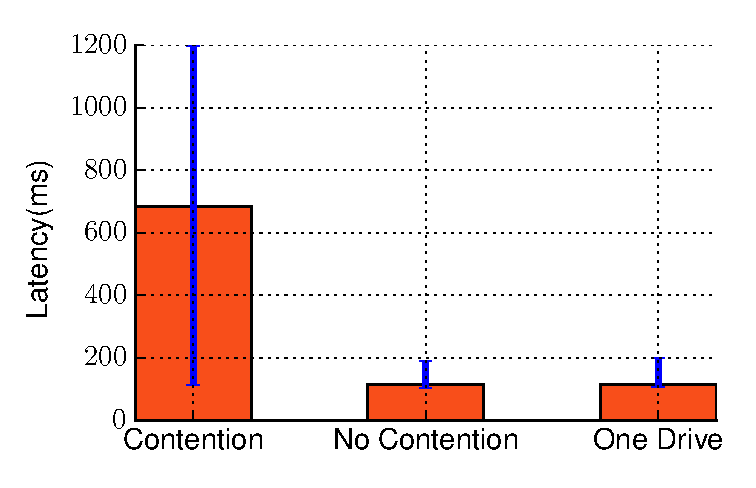
\includegraphics[width=0.40\textwidth]{plots/contention_bar}
      \caption{Contention vs No Contention}
      \label{fig:gizacontentionbar}
%  }
\end{figure}


%We evaluate the throughput of Giza in a local-area cluster. Figure xxx shows the result of a single Giza deployment for storing 4MB objects. The 24 ops per second equates to 144MB per second which is consistent with the 150MB per second cap for each Azure Virtual Machine. For each additional Giza node, we add three storage accounts. This is to deal with the current throughput cap per storage account, which is 200MB per second.  The keyspace is partitioned equally among sets of three storage accounts. Figure~\ref{fig:gizathroughput} depicts the throughput as we increase Giza nodes. Here, the throughput increases linearly. 

%\begin{figure*}
%\begin{tabular}{c|c|c|c|c|c}
%Giza Nodes & 1 & 2 & 3 & 4 & 5\\
%\hline
%ops/second & 24 & 34 & 49 & 73 & 96 \\
%MB/second & 144 & 204 & 294 & 438 & 576\\ 
%\end{tabular}
%\caption{Throughput result of local Giza cluster\label{fig:gizathroughput}} 
%\end{figure*}

%To set up CockroachDB, we use the same Azure virtual machine instances and run a single CockroachDB node. We followed the recommended production settings by the developers of CockroachDB when deploying these instances. For example, on the same virtual machine, we also run NTP to provide moderately accurate time to preserve data consistency. Other optimizations can be found on the CockroachDB website. We only benchmark CockraochDB against Giza in the 3 dc cluster scenario since we want the fault tolerance level to be the same for the comparisons.
%Since variability in latency is a factor when benchmarking cloud storage, we run all our experiments at approximately the same time.
%Since latency is an issue, we run all our experiments at around the same time.
%We experimented with different erasure coding schemes
% For all experiments, we deployed a single virtual machine (16 cores, 56 GB of RAM, 800 GB SSD, and gigabit ethernet) for each geographical region. We use the same virtual machines for setting up the Cassandra and CockroachDB clusters. The client issuing the requests runs on one of the virtual machine that is also part of the cluster. 
% To set up Giza, we also had to deployed both a table service and a blob service provided by the cloud service platform. The granularity of replication for these services varies from provider to provider but we always choose the replication level to match that of the regional replication. This means that as long as there’s no dc outage, the data would not be lost. For each data center, we run a Giza node frontend with the virtual machine. The Giza node can service requests from a client running in the virtual machine. In addition, requests to its local table and blob storage from other Giza nodes also go through the Giza node frontend in the form of an RPC call. This is to avoid unecessary WAN round trips when dealing with complicated table and blob storage operations. 
%\begin{figure}[t]
%  \centerline {
    \begin{subfigure}{0.45\textwidth}
      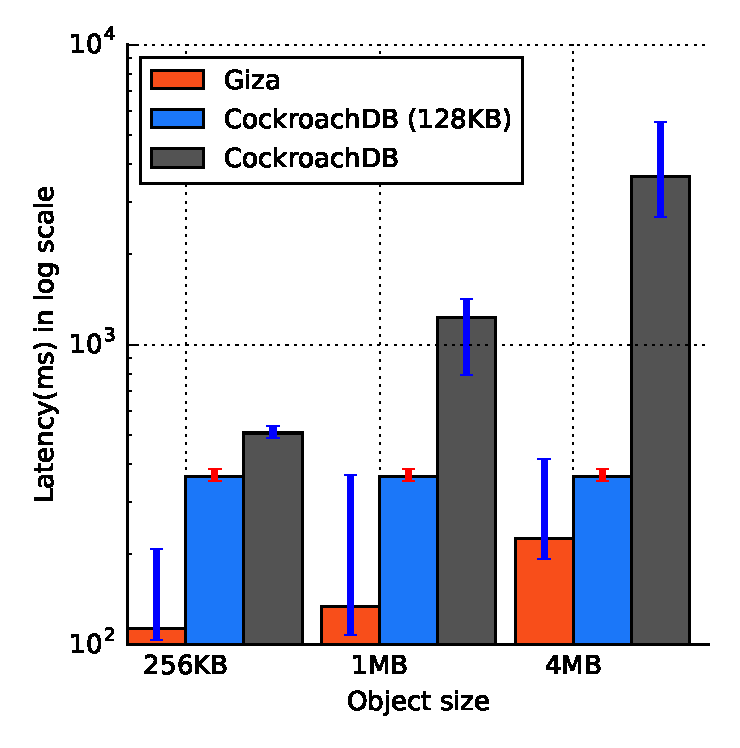
\includegraphics[width=\linewidth]{plots/giza_cock_put}

      % \placeholder{
      %   x-axis: \# clients / partition\\
      %   y-axis: cluster throughput\\
      %   lines: \name{}, OCC, 2PL, TAPIR\\
      %   }
%                \vspace{-1\baselineskip}
      \caption{Put}
      \label{fig:eval_cock_put}
    \end{subfigure}
%    \begin{subfigure}{0.33\textwidth}
%      \includegraphics[width=\linewidth]{figs/graphs/multi_dc/tpcc/tpcc_NEW_ORDER_tpcc_client_lat90.eps}
%
%      % \placeholder{
%      %   x-axis: \# clients / partition\\
%      %   y-axis: latency (median, p90, p99)\\
%      %   (maybe only show median and p99 or just median and report typical distribution)\\
%      %   lines: \name{}, OCC, 2PL, TAPIR\\
%      % }
%      \caption{90\% Latency}
%      \label{fig:geo_tpcc_latency}
%    \end{subfigure}
    \begin{subfigure}{0.45\textwidth}
      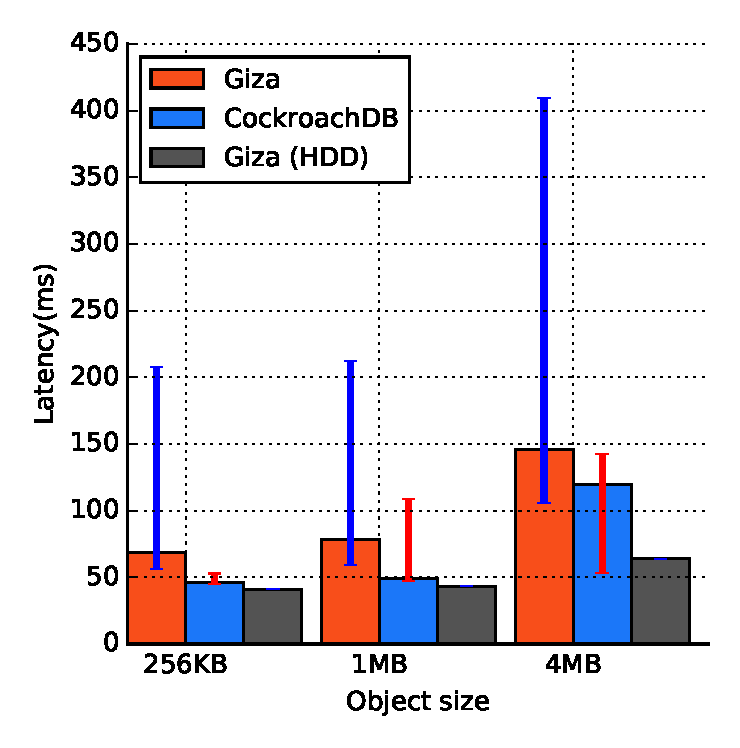
\includegraphics[width=\linewidth]{plots/giza_cock_get}

      % \placeholder{
      %   x-axis: \# clients / partition\\
      %   y-axis: commit rate\\
      %   lines: \name{}, OCC, 2PL, TAPIR\\
      % }
      %\includegraphics[width=\linewidth]{fig/kodiak/tpcc_mix_10_nlog_ct_cr.pdf}
%                \vspace{-1\baselineskip}
      \caption{Get}
      \label{fig:eval_cock_get}
    \end{subfigure}
%  }
  \caption{Performance for \name in different setups}
\end{figure}
% \begin{figure}[t]
% %  \centerline {
%       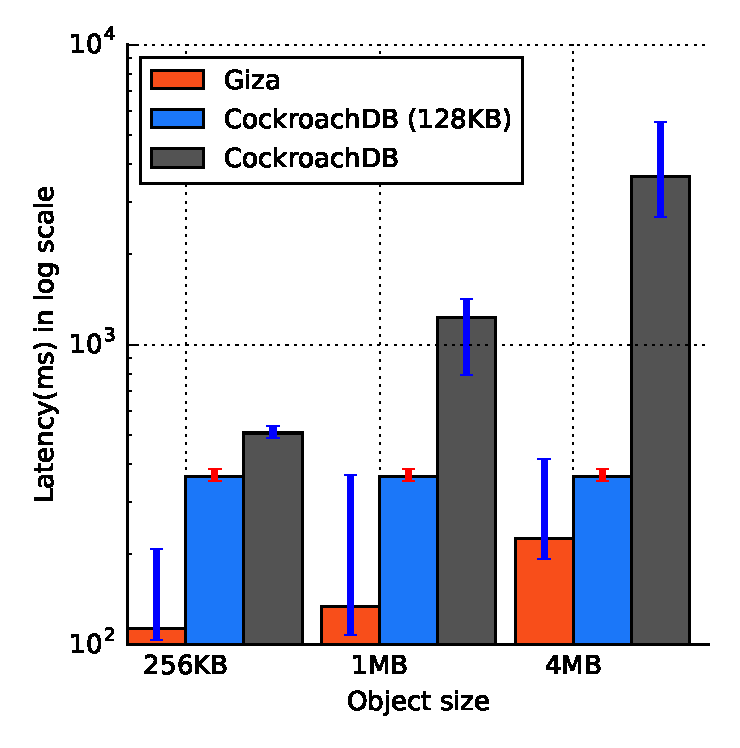
\includegraphics[width=\linewidth]{plots/giza_cock_put}
%       \caption{CockroachDB vs Giza Put with various object sizes}
%       \label{fig:eval_cock_put}
% %  }
% \end{figure}

% %\begin{figure}[t]
% %  \centerline {
% %      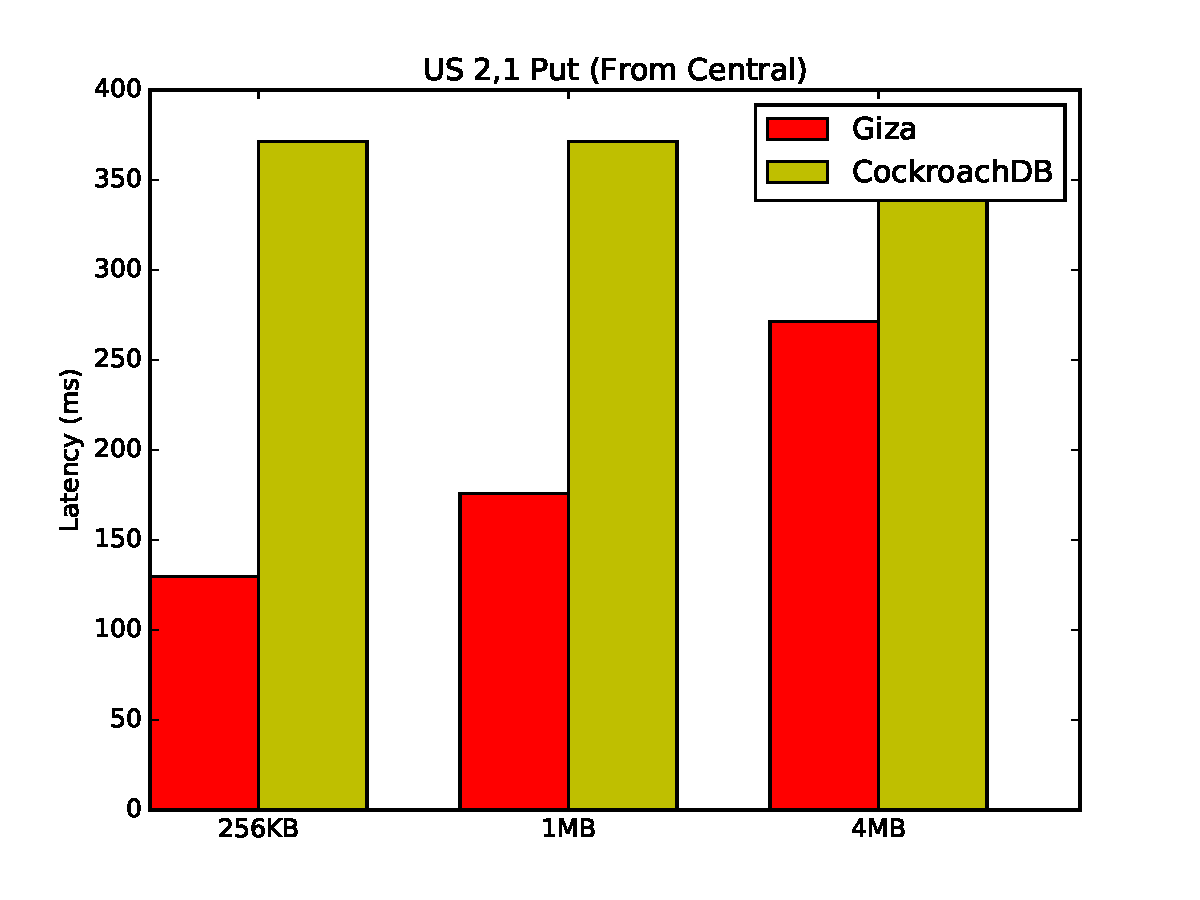
\includegraphics[width=\linewidth]{images/cockroach_vs_giza_put_128}
% %      \caption{CockroachDB vs Giza with various object sizes}
% %      \label{fig:eval_cock_put2}
% %  }
% %\end{figure}

% \begin{figure}[t]
% %  \centerline {
%       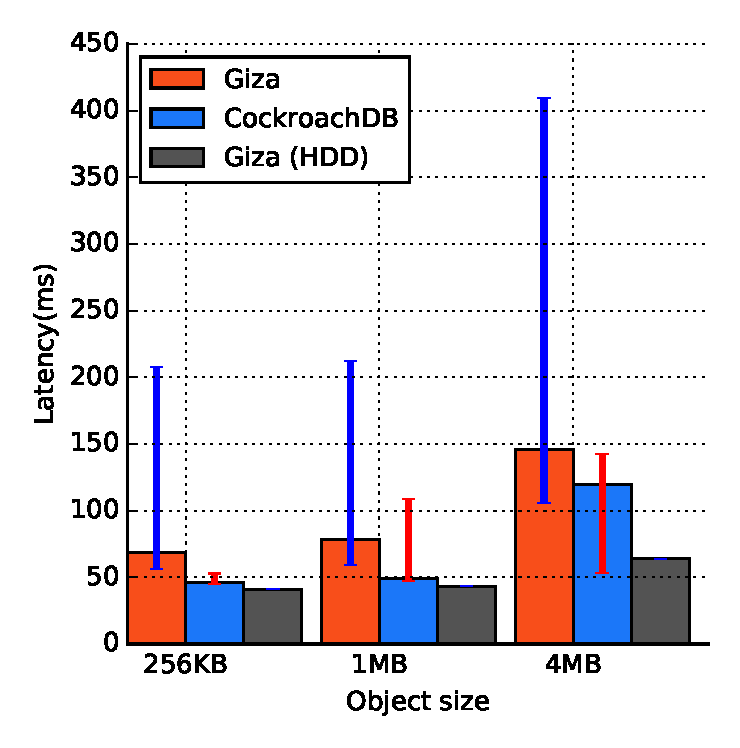
\includegraphics[width=\linewidth]{plots/giza_cock_get}
%       \caption{CockroachDB vs Giza Get with various object sizes}
%       \label{fig:eval_cock_get}
% %  }
% \end{figure}
%%% Local Variables:
%%% mode: latex
%%% TeX-master: "main"
%%% End:


%\sm {
%  In this section, I will have two graphs. One comparing Giza's full write path with CockroachDB's full replication. Another one is comparing the metadata path with cockroach db. This is to show, hopefully, that the fast paxos scheme is better. I will probably have 3 graphs each making request from one of the three datacenters. Due to multipaxos, there might be extra latency for cockroachdb's case.
%}
%We benchmark the performance of Giza with CockroachDB in two cases. In the first case, we use CockroachDB as a geo-replicating blah blah blah. Here is the result.
%In the second case, we used cockroachdb's transaction to simulate what we are doing with Giza. Blah blah blah, here is the result.
%64K $\sim$ 16MB

%X-axis: Value size
%Y-axis: 50\% Read latency

%X-axis: Value size
%Y-axis: 90\% Read latency

%X-axis: Value size
%Y-axis: 99\% Read latency

%Same for write

%[adding cpu results in a table]

% \subsection{Large object}
% 256MB $\sim$ 1GB

% X-axis: Value size
% Y-axis: Average Read latency

% X-axis: Value size
% Y-axis: Average Write latency


% \subsection{Contention}

% Fixed object size
% X-axis: zipf coefficient
% Y-axis: 50\%, 90\%, 99\% Read/Write Latency


% \subsection{Real workload}
% Table.


%%% Local Variables:
%%% mode: latex
%%% TeX-master: "main"
%%% End:

